\pdfoutput=1
\documentclass[12pt,letterpaper]{article}
\usepackage[margin=1in]{geometry}
\usepackage{setspace}
\usepackage{lineno}
\usepackage{graphicx}
\usepackage{booktabs}
\usepackage{caption}
\usepackage{amsmath}
\usepackage{array}
\usepackage{xurl}
\usepackage[hidelinks]{hyperref}
\usepackage[T1]{fontenc}
\usepackage[utf8]{inputenc}
\usepackage{lmodern}
\providecommand{\tightlist}{\setlength{\itemsep}{0pt}\setlength{\parskip}{0pt}}
\captionsetup{font=small,labelfont=bf}
\setcounter{secnumdepth}{0}
\setlength{\parindent}{0.25in}
\setlength{\parskip}{0pt}
\setlength{\emergencystretch}{3em}
\doublespacing
\linenumbers
\modulolinenumbers[1]
\begin{document}
\begin{center}
{\Large\bfseries A Two-Stage Product Audit for Strong-Motion Processing Windows}\\[1.5em]
Haoyu Zhou\\Qiang Ma\\
\vspace{0.35em}
Haoyu Zhou: Institute of Engineering Mechanics, China Earthquake Administration, Harbin, Heilongjiang, China\\Qiang Ma: Institute of Engineering Mechanics, China Earthquake Administration, Harbin, Heilongjiang, China\\
\vspace{0.35em}
Haoyu Zhou: zhouhaoyiu@gmail.com\\Qiang Ma: maqiang@iem.ac.cn\\
\vspace{0.35em}
Corresponding author: Qiang Ma; maqiang@iem.ac.cn\\Institute of Engineering Mechanics, China Earthquake Administration, 29 Xuefu Road, Nangang District, Harbin, Heilongjiang, China\\
\end{center}
\thispagestyle{plain}

\section{Abstract}\label{abstract}

The processing interval of an accelerogram determines which motion enters peak and response-spectrum products. Fixed intervals are convenient for archive production, yet the same duration can retain very different fractions of motion in different archives. We evaluated this problem with 44,674 three-component acceleration records from InstanceGM and K-NET and an external set of 6,107 PNWAccelerometers records. Every waveform received a common linear detrend and 0.1 Hz high-pass filter. The proposed offline audit has two stages. The first chooses the shortest waveform-derived candidate that retains at least 99\% of each component peak, at least 95\% of the three-component squared-motion integral, and all component peak times. The second checks the minimum component-wise retention of 5\%-damped pseudo-spectral acceleration (PSA) at 0.2, 1.0, and 3.0 s. A failed primary window is replaced by a padded 1\%-99\% cumulative-energy window; a second failure assigns the full record. A 42 s feature-onset window was unstable for 67.55\% of InstanceGM, 4.15\% of K-NET, and 86.56\% of PNW records under the first-stage criteria. The first-stage selection reduced the median main-set duration to 34.25 s, but 3.0 s PSA retention remained below 0.95 in 37.16\% of records. The spectral stage routed 60.08\% of the main set directly, 19.96\% to the energy-percentile window, and 19.96\% to the full record; the final median duration was 60.00 s. PNW routing was 34.42\%, 48.03\%, and 17.55\%, with a 150.01 s median. End-to-end tests at 0.05 and 0.10 Hz produced main-sample full-record rates of 22.81\% and 21.43\%. The audit supplies record-level evidence for fixed-window risk, spectral adequacy, and conservative fallback in offline strong-motion product production.

\section{Plain Language Summary}\label{plain-language-summary}

Strong-motion archives often store records with uniform durations because fixed windows simplify indexing and batch processing. A fixed duration does not guarantee that the retained samples are sufficient for every engineering product. We compare each candidate interval with its full record. Peak acceleration and energy provide a fast first check, followed by a response-spectrum check at three periods. Records that fail are assigned a longer energy-based interval or the full record. Tests on Italian, Japanese, and Pacific Northwest data show that suitable durations depend strongly on the archive. The output is a processing window accompanied by the measurements that justified it.

\section{Introduction}\label{introduction}

Strong-motion records support ground-motion models, shaking assessment, structural analysis, and postevent engineering review. Processing choices made before product calculation affect the resulting acceleration, velocity, displacement, duration, Fourier spectrum, and response spectrum. Filtering and baseline correction have received sustained attention because their consequences are visible in long-period products (Boore, 2001; Boore and Bommer, 2005; Douglas and Boore, 2011; Boore et al., 2012). The time interval retained for product calculation is another part of the same processing decision.

Strong-motion networks already use automated and reviewed processing systems. PRISM produces corrected time series, spectra, and intensity measures and supports record review (Jones et al., 2017). The USGS gmprocess system automates near-real-time ground-motion processing (Thompson et al., 2025). European RRSM and ESM services distribute rapid and reviewed strong-motion products (Cauzzi et al., 2016; Luzi et al., 2016). Similar product-generation systems have been developed for earthquake early-warning networks in China (Liu et al., 2025). Inocente and Maruyama (2026) jointly estimate P arrival and high-pass corner frequency for displacement-oriented strong-motion processing. These systems and methods need explicit processing parameters and quality flags that can be traced when products are regenerated.

Time-window selection has usually been designed for a target analysis. Kishida et al.~(2016) developed a semiautomated procedure for Fourier-amplitude spectra in NGA-West2. Perron et al.~(2018) selected phase and noise windows from arrival times, source duration, propagation time, and cumulative energy. Ryu et al.~(2025) compared preprocessing procedures and used a padded 1\%-99\% normalized Arias-intensity interval as one signal-window rule. These methods locate useful signal intervals. A production archive has an additional question: does a proposed interval preserve the quantities that the archive plans to publish?

Fixed windows remain common in public datasets. Their uniform shape simplifies storage and model development, and the original extraction rule may be adequate for the dataset's initial purpose. Product adequacy still requires a separate check when the same record is used to calculate peak and spectral measures. Event duration, path effects, basin response, trigger logic, and the length of available postevent motion all change how much information falls outside a fixed interval. A duration that works in one archive can truncate another.

This study formulates window choice as an offline product audit. The full acceleration record is available during archive preparation. Waveform features generate candidate intervals, and full-record products determine whether each candidate is acceptable. The method returns the shortest candidate that passes amplitude and energy checks, then applies a response-spectrum safeguard. Figure 1 summarizes the two-stage audit.

\begin{center}
\begin{minipage}{0.98\textwidth}
\centering

\includegraphics[width=0.95\textwidth]{figures/smqc_figure_01_workflow.pdf}
\captionof{figure}{Two-stage processing-window audit. The first stage retains the shortest candidate that preserves every component peak acceleration, relative three-component energy, and component peak times. The second stage checks 5\%-damped PSA at 0.2, 1.0, and 3.0 s and escalates failures to the padded 1\%-99\% cumulative-energy window or the full record.}
\noindent\textbf{Alt text:} Workflow from candidate windows through component-level amplitude and energy checks, PSA checks, and three possible output routes.
\label{fig:1}
\end{minipage}
\end{center}

The analysis addresses four questions. First, how strongly does fixed-window stability vary among archives and durations? Second, how much spectral risk remains after amplitude and energy screening? Third, what fraction of records requires an energy-percentile window or full-record fallback? Fourth, do the main findings persist under a second high-pass corner and in an external archive? The resulting method is intended for processing-window quality control in batch strong-motion product production.

\section{Data and Record Screening}\label{data-and-record-screening}

\subsection{Main archives}\label{main-archives}

The main analysis uses InstanceGM from the INSTANCE data family and K-NET records distributed by the National Research Institute for Earth Science and Disaster Resilience (NIED; see Data and Resources). INSTANCE provides Italian seismic waveforms and metadata for machine-learning and seismological applications (Michelini et al., 2021). K-NET is part of the nationwide Japanese strong-motion observation system (Aoi et al., 2004; Okada et al., 2004).

The initial worklist contained 45,652 records identified as acceleration data: 23,533 InstanceGM records in \(\mathrm{m\,s^{-2}}\) and 22,119 K-NET metadata rows. Waveforms were loaded before any product comparison. All InstanceGM records loaded successfully. The converted K-NET archive lacked waveform keys for 978 metadata rows, leaving 21,141 K-NET records. These rows remain in the availability log and do not enter rate denominators. The analyzed population contains 44,674 acceleration records (Table 1).

\begin{table}[!htbp]
\centering
\caption{Dataset flow for the 44,674-record acceleration audit. Duration is median [5th-95th percentile].}
\label{tab:dataset}
\begin{singlespace}
\footnotesize
\setlength{\tabcolsep}{3pt}
\begin{tabular*}{\textwidth}{@{\extracolsep{\fill}}lrrrrrlr@{}}
\toprule
Dataset & Candidates & Analyzed & Load errors & Events & Stations & Duration (s) & Median M \\
\midrule
InstanceGM & 23,533 & 23,533 & 0 & 8,811 & 299 & 120.00 [120.00-120.00] & 3.1 \\
K-NET & 22,119 & 21,141 & 978 & 1,528 & 917 & 119.00 [60.00-120.00] & 4.3 \\
\bottomrule
\end{tabular*}
\end{singlespace}
\end{table}

InstanceGM contributes 23,533 records from 8,811 events and 299 stations. K-NET contributes 21,141 records from 1,528 events and 917 stations. Median record durations are 120.00 and 119.00 s, respectively. The K-NET 5th and 95th duration percentiles are 60.00 and 120.00 s. Both archives have a median sampling rate of 100 Hz. Retention is calculated within each record, so constant amplitude-unit scaling does not affect the reported ratios.

Records are assigned to three descriptive magnitude groups: below M3, M3 to below M4, and M4 or larger. The groups support stratified reporting and deterministic sampling; they do not alter the window rule. InstanceGM contains 9,000, 9,000, and 5,533 records in these groups. K-NET contains 21, 5,647, and 15,473 records. The magnitude strata are listed in Table 2.

\begin{table}[!htbp]
\centering
\caption{Priority-stratum summary used in the waveform audit.}
\label{tab:priority}
\begin{singlespace}
\footnotesize
\setlength{\tabcolsep}{3pt}
\begin{tabular*}{0.82\textwidth}{@{\extracolsep{\fill}}llrrr@{}}
\toprule
Dataset & Stratum & Records & Median duration (s) & Median M \\
\midrule
InstanceGM & Low magnitude & 9,000 & 120.00 & 2.2 \\
InstanceGM & M3-M4 & 9,000 & 120.00 & 3.2 \\
InstanceGM & M4+ & 5,533 & 120.00 & 4.2 \\
K-NET & Low magnitude & 21 & 60.00 & 2.9 \\
K-NET & M3-M4 & 5,647 & 119.00 & 3.8 \\
K-NET & M4+ & 15,473 & 119.00 & 4.5 \\
\bottomrule
\end{tabular*}
\end{singlespace}
\end{table}

\subsection{External archive}\label{external-archive}

PNWAccelerometers provides an external check through the SeisBench interface (Ni et al., 2023; see Data and Resources). The evaluated subset contains 6,107 three-component acceleration records from 3,433 events and 168 stations. Its median duration is 150.01 s and median magnitude is 1.83. The three magnitude groups contain 5,563, 468, and 76 records. PNW records are reported separately because their event composition and archive construction differ from the main data.

\section{Methods}\label{methods}

\subsection{Common preprocessing}\label{common-preprocessing}

All acceleration records are linearly detrended and filtered with the same fourth-order, zero-phase Butterworth high-pass filter at 0.1 Hz. No resampling is applied. This setting holds preprocessing constant across archives. A deterministic 1,521-record sample is processed end to end at both 0.05 and 0.10 Hz. The sample contains up to 300 records from each dataset-magnitude group and includes every available member when a group has fewer than 300 records.

Let \(a_c(t)\) denote the filtered acceleration in component \(c\), with \(c=1,2,3\). Candidate generation uses the vector amplitude

\[
v(t)=\left(\sum_{c=1}^{3}a_c^2(t)\right)^{1/2}.
\]

The normalized cumulative squared-motion curve is the cumulative integral of \(v^2(t)\) divided by its full-record value. Its 1\% and 95\% times define an energy onset and energy end. A second onset is the first 0.1 s run that exceeds six robust standard deviations estimated from the first 3 s. The feature onset is the earlier finite value of the energy and threshold onsets.

\subsection{Candidate windows}\label{candidate-windows}

Each record has the following candidates: feature-onset windows extending 20, 40, 60, or 90 s after onset with 2 s of available preonset motion; a 40 s energy-onset window with the same preonset allowance; a feature-onset-to-energy-end interval with 3 s appended after the 95\% energy time; a cumulative-energy interval spanning 1\%-99\% with 15 s padding at both ends; and the full record. Intervals are clipped to the available samples. A 40 s post-P interval is calculated as a comparator. Catalog P is excluded from the primary selection.

The candidate set combines fixed durations with two waveform-adaptive endings. The 1\%-99\% interval is an Arias-type cumulative squared-acceleration measure summed over three components. The percentage times are unchanged by the constant factor in the conventional Arias-intensity definition (Arias, 1970).

\subsection{First-stage amplitude and energy audit}\label{first-stage-amplitude-and-energy-audit}

For a candidate interval \(I\) and full record \(F\), component-peak retention is

\[
r_A(I)=\min_c\frac{\max_{t\in I}|a_c(t)|}{\max_{t\in F}|a_c(t)|}.
\]

The squared-motion retention is

\[
r_E(I)=\frac{\sum_c\int_I a_c^2(t)\,dt}{\sum_c\int_F a_c^2(t)\,dt}.
\]

The candidate passes the first stage when \(r_A\geq0.99\), \(r_E\geq0.95\), and the time of the full-record absolute peak in every nonzero component lies inside the interval. The minimum component ratio prevents a large component from hiding peak loss in another component. The 0.99 and 0.95 thresholds are prespecified quality-control settings. The primary window is the shortest passing candidate that does not use catalog P. If no shorter candidate passes, the full record is selected.

\subsection{Response-spectrum safeguard}\label{response-spectrum-safeguard}

The first stage does not directly constrain structural response. For each component, we calculate 5\%-damped pseudo-spectral acceleration at periods \(\mathcal{T}=\{0.2,1.0,3.0\}\) s. The relative-displacement oscillator is

\[
\ddot u_c+2\zeta\omega\dot u_c+\omega^2u_c=-a_c(t),
\qquad PSA_c(T)=\omega^2\max_t|u_c(t)|,
\]

where \(\zeta=0.05\) and \(\omega=2\pi/T\). The continuous oscillator is discretized with a bilinear transform. Each input is followed by five zero-input oscillator cycles before the maximum is taken, so the record boundary does not truncate free vibration.

The spectral retention of interval \(I\) is

\[
r_S(T,I)=\min_c\frac{PSA_c(T,I)}{PSA_c(T,F)}.
\]

A primary interval passes when \(r_S(T,I)\geq0.95\) at every tested period. A failed interval is replaced by the padded 1\%-99\% cumulative-energy window and tested again. A second failure assigns the full record. This ordering yields three operational routes: primary, energy-window escalation, and full-record fallback. The final zero-failure property at the tested periods follows from the fallback rule; route fractions and output durations measure its operating cost.

\subsection{Evaluation}\label{evaluation}

Fixed-window instability is the fraction failing any first-stage criterion. Spectral failure is the fraction with \(r_S<0.95\) at a tested period. We report route fractions, median and 75th-percentile output duration, and results by archive and magnitude group. Spectral thresholds of 0.90, 0.95, and 0.98 quantify the relation between strictness and fallback. The end-to-end filter test reruns feature extraction, candidate construction, first-stage selection, PSA calculation, and final routing on the same 1,521 records.

The PNW SNR audit uses catalog timing only to define independent diagnostic intervals. Noise RMS is measured from P-22 to P-2 s. Signal RMS is measured from P to the later of P+20 s or S+20 s. Records are grouped at 3 and 10 dB before window outcomes are joined. This diagnostic compares the external result across weak and strong signals.

\section{Results}\label{results}

\subsection{Fixed-duration windows are archive dependent}\label{fixed-duration-windows-are-archive-dependent}

Figure 2 reports the fixed-duration sensitivity.

\begin{center}
\begin{minipage}{0.98\textwidth}
\centering

\includegraphics[width=0.95\textwidth]{figures/smqc_figure_02_fixed_window_failure.pdf}
\captionof{figure}{Fixed-duration sensitivity for InstanceGM, K-NET, and PNWAccelerometers. Values are instability rates for feature-onset windows ending 20, 40, 60, or 90 s after onset; each window also includes 2 s before onset.}
\noindent\textbf{Alt text:} Line plot comparing fixed-window instability across four post-onset durations and three archives.
\label{fig:2}
\end{minipage}
\end{center}

For feature-onset windows with 20, 40, 60, and 90 s of postonset motion, InstanceGM instability decreases from 94.36\% to 67.55\%, 50.10\%, and 32.90\%. K-NET decreases from 47.30\% to 4.15\%, 0.84\%, and 0.15\%. PNW remains high at 91.01\%, 86.56\%, 82.71\%, and 75.90\%.

The failure fields show what is lost at 40 s. In InstanceGM, 15,896 of 23,533 windows fail; 15,847 have insufficient energy retention, 6,269 omit at least one component peak time, and 6,170 fall below the component-peak ratio. K-NET has 877 failures, all with insufficient energy retention; 46 omit a component peak. PNW has 5,286 failures, all with insufficient energy retention and 4,980 with a component peak outside the window. These counts can overlap because one window may fail several checks.

\subsection{Amplitude-energy selection leaves period-dependent loss}\label{amplitude-energy-selection-leaves-period-dependent-loss}

Before the spectral stage, the primary selector assigns only 37 InstanceGM records, no K-NET records, and one PNW record to the full interval. Median primary durations are 62.00 s for InstanceGM, 22.00 s for K-NET, and 142.37 s for PNW. The combined main-set median is 34.25 s.

Short primary intervals do not preserve every spectral ordinate. Across the main set, 0.2, 1.0, and 3.0 s PSA failure rates are 0.11\%, 7.59\%, and 37.16\%. The corresponding 42 s fixed-window rates are 11.85\%, 26.80\%, and 58.30\%. Figure 4 shows the corresponding PSA failures.

\begin{center}
\begin{minipage}{0.98\textwidth}
\centering

\includegraphics[width=0.95\textwidth]{figures/smqc_figure_04_product_impact_recovery.pdf}
\captionof{figure}{PSA-retention failures at 0.2, 1.0, and 3.0 s for the 42 s fixed window, the primary amplitude-energy window, and the final safeguarded output. The safeguarded output meets the 0.95 threshold at every tested period by construction, with full-record fallback retained in the denominator.}
\noindent\textbf{Alt text:} Grouped bars compare PSA-retention failures before and after the spectral safeguard for all records and each primary archive.
\label{fig:4}
\end{minipage}
\end{center}

The growing difference with period explains the need for a product-specific second stage.

\subsection{Spectral routing and output duration}\label{spectral-routing-and-output-duration}

Figure 3 reports the final routing and duration.

\begin{center}
\begin{minipage}{0.98\textwidth}
\centering

\includegraphics[width=0.95\textwidth]{figures/smqc_figure_03_selector_duration_fallback.pdf}
\captionof{figure}{Final processing routes and window durations after the spectral safeguard. Records retain the primary window, escalate to the padded 1\%-99\% cumulative-energy window, or fall back to the full record. Error bars show the 75th percentile above the median duration.}
\noindent\textbf{Alt text:} Stacked bars show three audit routes and adjacent bars show median and 75th-percentile output durations for three archives.
\label{fig:3}
\end{minipage}
\end{center}

In the main set, 60.08\% of records retain the primary interval, 19.96\% move to the padded energy-percentile interval, and 19.96\% use the full record. The final median and 75th-percentile durations are 60.00 and 110.23 s. Table 3 lists the routing percentages.

\begin{table}[!htbp]
\centering
\caption{Final routes after component-level peak, energy, and response-spectrum audits.}
\label{tab:stability}
\begin{singlespace}
\footnotesize
\setlength{\tabcolsep}{3pt}
\begin{tabular}{lrrrrrr}
\toprule
Dataset & Records & Primary (\%) & Energy window (\%) & Full record (\%) & Median (s) & p75 (s) \\
\midrule
InstanceGM & 23,533 & 69.26 & 24.97 & 5.77 & 92.00 & 110.50 \\
K-NET & 21,141 & 49.86 & 14.38 & 35.76 & 44.81 & 81.00 \\
PNW & 6,107 & 34.42 & 48.03 & 17.55 & 150.01 & 150.01 \\
\bottomrule
\end{tabular}
\end{singlespace}
\end{table}

InstanceGM routes 69.26\% to the primary interval, 24.97\% to the energy-percentile interval, and 5.77\% to the full record; its median final duration is 92.00 s. K-NET routes 49.86\%, 14.38\%, and 35.76\%, with a 44.81 s median. PNW routes 34.42\%, 48.03\%, and 17.55\%; its median and 75th percentile both equal 150.01 s. The method preserves the PNW full duration for at least half of the records because the shorter candidates frequently miss the tested spectrum.

The tested spectral threshold controls this routing. At thresholds of 0.90, 0.95, and 0.98, main-set full-record rates are 18.28\%, 19.96\%, and 21.65\%; primary acceptance is 66.01\%, 60.08\%, and 53.13\%. Median final duration is 60.00 s at 0.90 and 0.95 and 65.18 s at 0.98. PNW full-record rates are 16.70\%, 17.55\%, and 18.39\% over the same thresholds.

\subsection{Preprocessing and external diagnostics}\label{preprocessing-and-external-diagnostics}

Figure 5 reports this preprocessing sensitivity.

\begin{center}
\begin{minipage}{0.98\textwidth}
\centering
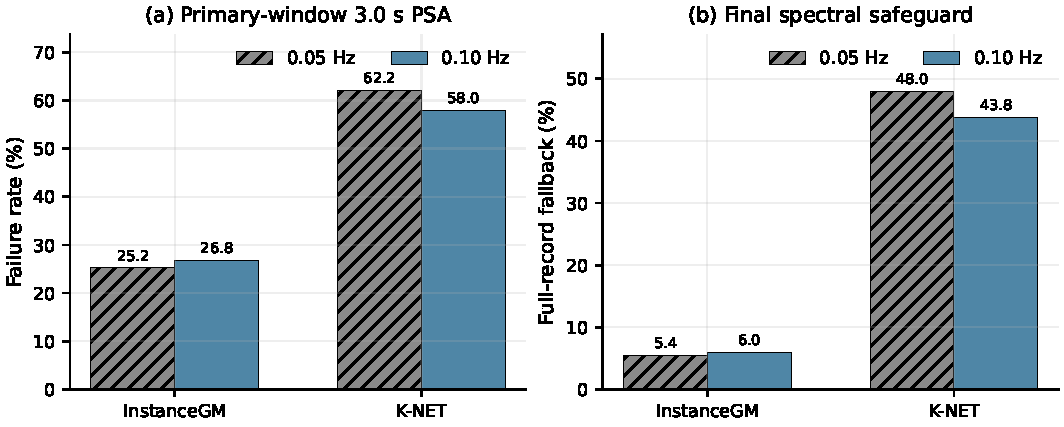
\includegraphics[width=0.95\textwidth]{figures/smqc_figure_05_filter_sensitivity.pdf}
\captionof{figure}{High-pass-filter sensitivity on the same stratified 1,521-record sample. Panels compare primary-window 3.0 s PSA failures and final full-record fallback under 0.05 and 0.10 Hz preprocessing.}
\noindent\textbf{Alt text:} Paired bars compare long-period PSA failures and conservative fallback rates at two high-pass corners.
\label{fig:5}
\end{minipage}
\end{center}

In the end-to-end 1,521-record comparison, 3.0 s primary-window failure is 40.30\% at 0.05 Hz and 39.51\% at 0.10 Hz. Final full-record rates are 22.81\% and 21.43\%, and median final durations are 69.00 and 66.59 s. InstanceGM full-record rates are 5.44\% and 6.00\%. K-NET rates are 47.99\% and 43.80\%. The archive contrast and the need for a spectral stage persist under both corners.

Figure 6 reports the SNR-stratified results.

\begin{center}
\begin{minipage}{0.98\textwidth}
\centering

\includegraphics[width=0.95\textwidth]{figures/smqc_figure_06_response_spectrum_retention.pdf}
\captionof{figure}{PNWAccelerometers results by a result-blind RMS signal-to-noise ratio computed from catalog-timed pre-event and signal intervals. Panels show fixed-window instability, primary-window 3.0 s PSA failure, and final full-record fallback.}
\noindent\textbf{Alt text:} Three bar charts compare fixed-window, primary-spectrum, and final-fallback behavior across three PNW signal-to-noise groups.
\label{fig:6}
\end{minipage}
\end{center}

PNW fixed-window instability is 99.15\%, 99.69\%, and 70.32\% in the below-3, 3-10, and at-least-10 dB groups. Primary 3.0 s PSA failure is 50.81\%, 63.34\%, and 66.67\%. Final full-record fallback is 0.68\%, 0.76\%, and 38.65\%. The strongest SNR group retains the highest full-record rate, placing the external finding in strong-signal records as well. Its median magnitude is also higher (2.22 versus 1.49 and 1.74); the present stratification cannot separate magnitude, duration, and path effects.

\section{Discussion}\label{discussion}

\subsection{Why fixed public windows still need an audit}\label{why-fixed-public-windows-still-need-an-audit}

Uniform windows solve an archive-format problem. They give every record the same tensor shape and simplify bulk access. Product-window adequacy is a different property. InstanceGM and PNW contain substantial motion beyond 40 s for many records, while most K-NET records pass the first-stage checks at that duration. Increasing all windows to 90 s reduces failure in each archive but leaves 32.90\% of InstanceGM and 75.90\% of PNW unstable and stores unnecessary samples for many K-NET records.

The archive contrast can arise from several mechanisms. Record extraction rules set the available preevent and postevent motion. Trigger and detrigger settings determine how much coda is retained. Source magnitude, path length, basin response, and late arrivals change physical duration. Noise contributes to cumulative-energy timing in weak records, a known limitation of energy-based endings (Perron et al., 2018; Ryu et al., 2025). The present audit measures their combined effect on products; separating the individual mechanisms requires archive-specific acquisition and trigger metadata.

\subsection{Why the spectral stage changes the result}\label{why-the-spectral-stage-changes-the-result}

Peak acceleration and total squared motion are scalar summaries. A candidate can retain both and still alter the maximum response of a damped oscillator. The main-set 3.0 s failure rate of 37.16\% after first-stage selection demonstrates this distinction. The added spectral check directly matches the stated product requirement.

The final 0\% failure rate at 0.2, 1.0, and 3.0 s is a quality-control guarantee produced by the rule. Its substantive results are the escalation rate, fallback rate, and final duration required to meet that guarantee. The guarantee covers the stated preprocessing, damping, periods, component rule, and retention threshold. Products at longer periods or with different damping need their own audit periods. The 0.05/0.10 Hz comparison also shows that processing settings belong in the audit record.

\subsection{Use in strong-motion product production}\label{use-in-strong-motion-product-production}

The method fits an offline production step after waveform retrieval and before product export. Each record receives a candidate source, start and end samples, component-peak retention, energy retention, peak-time status, three PSA retention values, final route, and the preprocessing configuration. Product tables can retain these fields as provenance. Archive updates can be rerun with the same thresholds, and records assigned to the full interval can be inspected without changing the accepted records.

The PNW result illustrates a conservative outcome. A median final duration equal to the available 150.01 s means the tested shorter intervals do not support the selected product target for much of this archive. The audit reports that cost directly. The spectral stage exposes product loss left unresolved by onset and energy checks.

This study uses the available record as the product reference. A full record can contain noise, secondary events, or recording artifacts, and those features may affect its spectrum. The SNR analysis addresses one part of that concern. Record-level signal classification remains a separate production requirement. Future tests can pair the current retention fields with established waveform-quality screens (Douglas, 2003; Bellagamba et al., 2019) and operator-reviewed cases. The current results establish product retention and routing behavior; operator time savings require a separate workflow study.

\section{Conclusions}\label{conclusions}

A fixed processing duration does not transfer uniformly among InstanceGM, K-NET, and PNWAccelerometers. At 40 s after feature onset, first-stage instability ranges from 4.15\% in K-NET to 86.56\% in PNW. Duration alone is insufficient as a cross-archive quality rule.

The amplitude-energy stage supplies compact candidates and a transparent first screen. Its main-set median is 34.25 s, while 37.16\% of records still lose more than 5\% of 3.0 s PSA in at least one component. The spectral stage resolves this product mismatch through energy-window escalation and full-record fallback. At the 0.95 setting, the main routes are 60.08\% primary, 19.96\% energy-window, and 19.96\% full record.

The method provides a reproducible processing-window audit for offline strong-motion product production. Its output records why a window was accepted, when a longer interval was required, and which preprocessing and spectral criteria were applied.

\section{Data and Resources}\label{data-and-resources}

InstanceGM/INSTANCE data were accessed through the INSTANCE data system at https://doi.org/10.13127/INSTANCE on 16 June 2026. K-NET data were accessed from NIED at https://doi.org/10.17598/NIED.0004 on 16 June 2026. PNWAccelerometers data were accessed through the SeisBench data interface on 18 June 2026; the dataset is described by Ni et al.~(2023), https://doi.org/10.26443/seismica.v2i1.368.

Code, tests, derived audit tables, figure source data, and reproduction commands are archived at https://github.com/zhouhaoyiu/strong-motion-product-window-qc/releases/tag/v0.2.0 (last accessed July 2026). Raw waveforms are not redistributed and remain subject to provider terms. Source code is released under the MIT License. Derived tables, figures, and documentation are released under CC BY 4.0. OpenAI Codex desktop application version 26.707.31428 assisted with code editing, consistency checks, and language editing. Reported values were generated by the archived scripts. The authors inspected the code and compared the manuscript values with the archived outputs, then reviewed the figures, scientific interpretation, and final text.

\section{Acknowledgments}\label{acknowledgments}

The authors thank the INSTANCE, NIED K-NET, PNWAccelerometers, and SeisBench teams for maintaining public waveform resources. This research received no external funding.

\section{Declaration of Competing Interests}\label{declaration-of-competing-interests}

The authors declare no competing interests.

\section{References}\label{references}

Aoi, S., T. Kunugi, and H. Fujiwara (2004). Strong-motion seismograph network operated by NIED: K-NET and KiK-net, \emph{J. Japan Assoc. Earthq. Eng.} 4, no. 3, 65-74, doi: 10.5610/jaee.4.3\_65.

Arias, A. (1970). A measure of earthquake intensity, in \emph{Seismic Design for Nuclear Power Plants}, R. J. Hansen (Editor), MIT Press, Cambridge, Massachusetts, 438-483.

Bellagamba, X., R. Lee, and B. A. Bradley (2019). A neural network for automated quality screening of ground motion records from small magnitude earthquakes, \emph{Earthq. Spectra} 35, no. 4, 1637-1661, doi: 10.1193/122118EQS292M.

Boore, D. M. (2001). Effect of baseline corrections on displacements and response spectra for several recordings of the 1999 Chi-Chi, Taiwan, earthquake, \emph{Bull. Seismol. Soc. Am.} 91, no. 5, 1199-1211, doi: 10.1785/0120000703.

Boore, D. M., A. Azari Sisi, and S. Akkar (2012). Using pad-stripped acausally filtered strong-motion data, \emph{Bull. Seismol. Soc. Am.} 102, no. 2, 751-760, doi: 10.1785/0120110222.

Boore, D. M., and J. J. Bommer (2005). Processing of strong-motion accelerograms: needs, options and consequences, \emph{Soil Dyn. Earthq. Eng.} 25, no. 2, 93-115, doi: 10.1016/j.soildyn.2004.10.007.

Cauzzi, C., R. Sleeman, J. Clinton, J. D. Ballesta, O. Galanis, and P. Kastli (2016). Introducing the European Rapid Raw Strong-Motion database, \emph{Seismol. Res. Lett.} 87, no. 4, 977-986, doi: 10.1785/0220150271.

Douglas, J. (2003). What is a poor quality strong-motion record?, \emph{Bull. Earthq. Eng.} 1, no. 1, 141-156, doi: 10.1023/A:1024861528201.

Douglas, J., and D. M. Boore (2011). High-frequency filtering of strong-motion records, \emph{Bull. Earthq. Eng.} 9, no. 2, 395-409, doi: 10.1007/s10518-010-9208-4.

Inocente, I., and Y. Maruyama (2026). Automated strong-motion record processing via deep learning-based simultaneous P-wave identification and high-pass corner-frequency selection, \emph{Seism. Rec.} 6, no. 2, 219-229, doi: 10.1785/0320260007.

Jones, J. M., E. Kalkan, C. D. Stephens, and P. Ng (2017). PRISM software: Processing and Review Interface for Strong-Motion Data, \emph{Seismol. Res. Lett.} 88, no. 3, 851-866, doi: 10.1785/0220160200.

Kishida, T., O.-J. Ktenidou, R. B. Darragh, and W. J. Silva (2016). \emph{Semi-Automated Procedure for Windowing Time Series and Computing Fourier Amplitude Spectra for the NGA-West2 Database}, PEER Report 2016/02, Pacific Earthquake Engineering Research Center, University of California, Berkeley.

Liu, Y., L. Zou, Q. Zhang, and X. Li (2025). Strong-motion data processing and product generation system for earthquake early warning network, \emph{Appl. Syst. Innov.} 8, no. 6, 172, doi: 10.3390/asi8060172.

Luzi, L., R. Puglia, E. Russo, M. D'Amico, C. Felicetta, F. Pacor, G. Lanzano, U. Ceken, J. Clinton, G. Costa, L. Duni, E. Farzanegan, P. Gueguen, C. Ionescu, I. Kalogeras, et al.~(2016). The Engineering Strong-Motion Database: A platform to access pan-European accelerometric data, \emph{Seismol. Res. Lett.} 87, no. 4, 987-997, doi: 10.1785/0220150278.

Michelini, A., S. Cianetti, S. Gaviano, C. Giunchi, D. Jozinovic, and V. Lauciani (2021). INSTANCE: The Italian seismic dataset for machine learning, \emph{Earth Syst. Sci. Data} 13, no. 12, 5509-5544, doi: 10.5194/essd-13-5509-2021.

Ni, Y., A. Hutko, F. Skene, M. Denolle, S. Malone, P. Bodin, R. Hartog, and A. Wright (2023). Curated Pacific Northwest AI-ready Seismic Dataset, \emph{Seismica} 2, no. 1, doi: 10.26443/seismica.v2i1.368.

Okada, Y., K. Kasahara, S. Hori, K. Obara, S. Sekiguchi, H. Fujiwara, and A. Yamamoto (2004). Recent progress of seismic observation networks in Japan: Hi-net, F-net, K-NET and KiK-net, \emph{Earth Planets Space} 56, no. 8, xv-xxviii, doi: 10.1186/BF03353076.

Perron, V., A. Laurendeau, F. Hollender, P.-Y. Bard, C. Gelis, P. Traversa, and S. Drouet (2018). Selecting time windows of seismic phases and noise for engineering seismology applications: a versatile methodology and algorithm, \emph{Bull. Earthq. Eng.} 16, no. 6, 2211-2225, doi: 10.1007/s10518-017-0131-9.

Ryu, B., S. Bang, and D. Kwak (2025). Earthquake ground motion characteristics as a function of a preprocessing procedure, \emph{Appl. Sci.} 15, no. 23, 12453, doi: 10.3390/app152312453.

Thompson, E. M., M. Hearne, B. T. Aagaard, J. M. Rekoske, C. B. Worden, M. P. Moschetti, H. E. Hunsinger, G. C. Ferragut, G. A. Parker, J. A. Smith, K. K. Smith, and A. R. Kottke (2025). Automated, near real-time ground-motion processing at the U.S. Geological Survey, \emph{Seismol. Res. Lett.} 96, no. 1, 538-553, doi: 10.1785/0220240021.

\section{Corresponding Author}\label{corresponding-author}

Correspondence should be addressed to Qiang Ma, Institute of Engineering Mechanics, China Earthquake Administration, 29 Xuefu Road, Nangang District, Harbin, Heilongjiang, China; email: maqiang@iem.ac.cn.


\end{document}
